\documentclass[11pt,a4paper]{article}
\usepackage[margin=1in]{geometry}
\usepackage[T1]{fontenc}
\usepackage[utf8]{inputenc}
\usepackage{lmodern}
\usepackage{hyperref}
\usepackage{enumitem}
\usepackage{xurl}
\usepackage{tikz}
\usepackage{float}
\usetikzlibrary{arrows.meta, positioning, shapes.geometric}
\hypersetup{colorlinks=true,linkcolor=blue,urlcolor=blue}
\newcommand{\codepath}[1]{\path{#1}}
\tikzset{
  box/.style={rectangle,draw,rounded corners,align=center,inner sep=3pt,minimum width=44mm},
  decision/.style={diamond,draw,aspect=2.2,align=center,inner sep=2pt},
  line/.style={-Latex}
}

\title{Phase-2 QEMU: Deliverable 9 (CI Integration)}
\author{SIT Engine Documentation}
\date{\today}

\begin{document}
\maketitle

\section{Technical Description}
CI integration for QEMU runs deterministic parser/replay/invariant gates automatically and blocks merges on regressions.

\section{Implementation Fulfillment}
CI uses executable gates from \codepath{Phase-2/tests/} and cross-target smoke from \codepath{Phase-2/run_cross_target_suite.py}. 

\section{Design \& Architecture}
\subsection*{Function Attributes}
\begin{itemize}[leftmargin=*]
  \item \texttt{check\_adapter\_fixtures.main()}: Inputs=fixture traces + expected snapshots; Outputs=parser stability verdict; Side effects=detects parser drift; Failure modes=snapshot mismatch.
  \item \texttt{run\_golden\_suite.main()}: Inputs=manifest + outdir; Outputs=replay outputs/verdict; Side effects=replay correctness gate; Failure modes=replay failure.
  \item \texttt{check\_invariants.main()}: Inputs=run\_windows.csv; Outputs=invariant verdict; Side effects=enforces engine-level constraints; Failure modes=invariant violation.
  \item \texttt{check\_determinism.main()}: Inputs=rerun outputs; Outputs=determinism verdict; Side effects=asserts byte-identical reruns; Failure modes=hash mismatch.
  \item \texttt{run\_cross\_target\_suite.main()}: Inputs=target/workload matrix; Outputs=smoke verdict; Side effects=checks integration breadth; Failure modes=target/tool failures.
\end{itemize}
\subsection*{Function Execution Details}
\begin{enumerate}[leftmargin=*]
  \item \texttt{check\_adapter\_fixtures.main()}
  \begin{itemize}[leftmargin=*]
    \item Input attributes: fixture traces + expected snapshots.
    \item Processing flow: detects parser drift.
    \item Output attributes: parser stability verdict.
    \item Failure behavior: snapshot mismatch.
  \end{itemize}
  \item \texttt{run\_golden\_suite.main()}
  \begin{itemize}[leftmargin=*]
    \item Input attributes: manifest + outdir.
    \item Processing flow: replay correctness gate.
    \item Output attributes: replay outputs/verdict.
    \item Failure behavior: replay failure.
  \end{itemize}
  \item \texttt{check\_invariants.main()}
  \begin{itemize}[leftmargin=*]
    \item Input attributes: run\_windows.csv.
    \item Processing flow: enforces engine-level constraints.
    \item Output attributes: invariant verdict.
    \item Failure behavior: invariant violation.
  \end{itemize}
  \item \texttt{check\_determinism.main()}
  \begin{itemize}[leftmargin=*]
    \item Input attributes: rerun outputs.
    \item Processing flow: asserts byte-identical reruns.
    \item Output attributes: determinism verdict.
    \item Failure behavior: hash mismatch.
  \end{itemize}
  \item \texttt{run\_cross\_target\_suite.main()}
  \begin{itemize}[leftmargin=*]
    \item Input attributes: target/workload matrix.
    \item Processing flow: checks integration breadth.
    \item Output attributes: smoke verdict.
    \item Failure behavior: target/tool failures.
  \end{itemize}
\end{enumerate}


\subsection*{Diagram A: End-to-End Design Flow}
\begin{figure}[H]
\centering
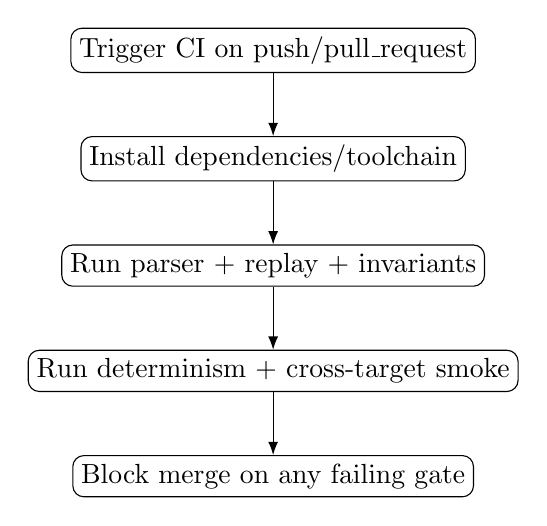
\begin{tikzpicture}[node distance=8mm and 12mm]
\node[box] (a) {Trigger CI on push/pull\_request};
\node[box, below=of a] (b) {Install dependencies/toolchain};
\node[box, below=of b] (c) {Run parser + replay + invariants};
\node[box, below=of c] (d) {Run determinism + cross-target smoke};
\node[box, below=of d] (e) {Block merge on any failing gate};
\draw[line] (a) -- (b);
\draw[line] (b) -- (c);
\draw[line] (c) -- (d);
\draw[line] (d) -- (e);
\end{tikzpicture}
\caption{QEMU Deliverable 09: End-to-End Design Flow}
\end{figure}

\subsection*{Diagram B: Function Interaction and Attribute Flow}
\begin{figure}[H]
\centering
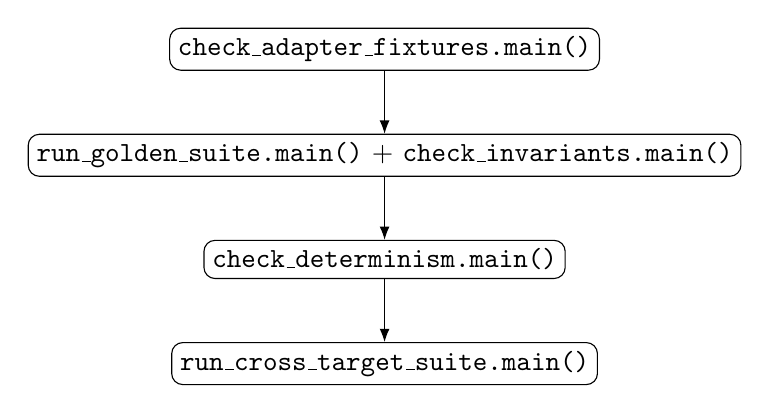
\begin{tikzpicture}[node distance=8mm and 12mm]
\node[box] (fa) {\texttt{check\_adapter\_fixtures.main()}};
\node[box, below=of fa] (fb) {\texttt{run\_golden\_suite.main()} + \texttt{check\_invariants.main()}};
\node[box, below=of fb] (fc) {\texttt{check\_determinism.main()}};
\node[box, below=of fc] (fd) {\texttt{run\_cross\_target\_suite.main()}};
\draw[line] (fa) -- (fb);
\draw[line] (fb) -- (fc);
\draw[line] (fc) -- (fd);
\end{tikzpicture}
\caption{QEMU Deliverable 09: Function Interaction and Attribute Flow}
\end{figure}

\end{document}
